\newpage
\setlength{\parskip}{1em}
\section{Annex}
\label{sec:annex}
\subsection{Kalman Filter equations}
Nomenclature provided by \textit{Wikipedia}:

$F_k$: transition matrix

$H_k$: measurement model

$Q_k$: process covariance matrix

$R_k$: measurement covariance matrix

$B_k$: control-input model

$u_k$: control vector

$w_k$: process noise (assumed normally distributed)

\textbf{Equations for prediction step:}

Predicted (a priori) state estimate:

	{\displaystyle {\hat {\mathbf {x} }}_{k\mid k-1}=\mathbf {F} _{k}{\hat {\mathbf {x} }}_{k-1\mid k-1}+\mathbf {B} _{k}\mathbf {u} _{k}} {\displaystyle {\hat {\mathbf {x} }}_{k\mid k-1}=\mathbf {F} _{k}{\hat {\mathbf {x} }}_{k-1\mid k-1}+\mathbf {B} _{k}\mathbf {u} _{k}}
	
Predicted (a priori) estimate covariance:

	{\displaystyle \mathbf {P} _{k\mid k-1}=\mathbf {F} _{k}\mathbf {P} _{k-1\mid k-1}\mathbf {F} _{k}^{\mathrm {T} }+\mathbf {Q} _{k}} {\displaystyle \mathbf {P} _{k\mid k-1}=\mathbf {F} _{k}\mathbf {P} _{k-1\mid k-1}\mathbf {F} _{k}^{\mathrm {T} }+\mathbf {Q} _{k}}
	
\textbf{Equations for update step:}

Innovation measurement

	{\displaystyle {\tilde {\mathbf {y} }}_{k}=\mathbf {z} _{k}-\mathbf {H} _{k}{\hat {\mathbf {x} }}_{k\mid k-1}} {\tilde {\mathbf {y} }}_{k}=\mathbf {z} _{k}-\mathbf {H} _{k}{\hat {\mathbf {x} }}_{k\mid k-1}
	
Innovation covariance

	{\displaystyle \mathbf {S} _{k}=\mathbf {R} _{k}+\mathbf {H} _{k}\mathbf {P} _{k\mid k-1}\mathbf {H} _{k}^{\mathrm {T} }} {\displaystyle \mathbf {S} _{k}=\mathbf {R} _{k}+\mathbf {H} _{k}\mathbf {P} _{k\mid k-1}\mathbf {H} _{k}^{\mathrm {T} }}
	
Optimal Kalman gain

	{\displaystyle \mathbf {K} _{k}=\mathbf {P} _{k\mid k-1}\mathbf {H} _{k}^{\mathrm {T} }\mathbf {S} _{k}^{-1}} {\displaystyle \mathbf {K} _{k}=\mathbf {P} _{k\mid k-1}\mathbf {H} _{k}^{\mathrm {T} }\mathbf {S} _{k}^{-1}}

Updated (a posteriori) state estimate

	{\displaystyle {\hat {\mathbf {x} }}_{k\mid k}={\hat {\mathbf {x} }}_{k\mid k-1}+\mathbf {K} _{k}{\tilde {\mathbf {y} }}_{k}} {\hat {\mathbf {x} }}_{k\mid k}={\hat {\mathbf {x} }}_{k\mid k-1}+\mathbf {K} _{k}{\tilde {\mathbf {y} }}_{k}

Updated (a posteriori) estimate covariance

	{\displaystyle \mathbf {P} _{k|k}=(\mathbf {I} -\mathbf {K} _{k}\mathbf {H} _{k})\mathbf {P} _{k|k-1}(\mathbf {I} -\mathbf {K} _{k}\mathbf {H} _{k})^{T}+\mathbf {K} _{k}\mathbf {R} _{k}\mathbf {K} _{k}^{T}}
	
Measurement residual

	{\displaystyle {\tilde {\mathbf {y} }}_{k\mid k}=\mathbf {z} _{k}-\mathbf {H} _{k}{\hat {\mathbf {x} }}_{k\mid k}} {\displaystyle {\tilde {\mathbf {y} }}_{k\mid k}=\mathbf {z} _{k}-\mathbf {H} _{k}{\hat {\mathbf {x} }}_{k\mid k}}
\newpage
\subsection{Kalman Filter performance for different noise levels}
In the dynamics environment:
\begin{figure}[ht!]
\centering
\captionsetup{justification=centering,margin=1cm}
\resizebox{\textwidth}{!}{\begin{tabular}{cc}
%\hline
\subf{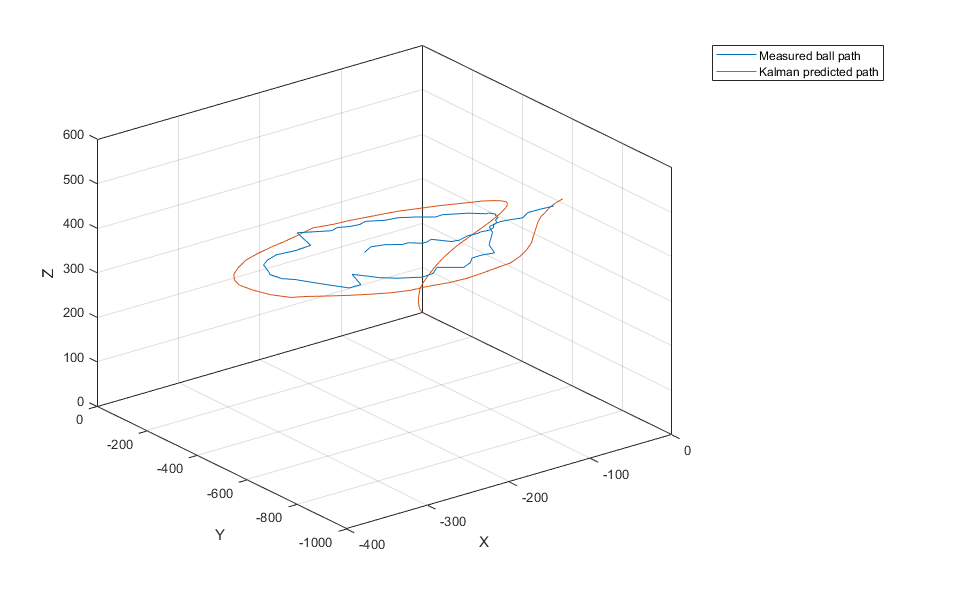
\includegraphics[width=60mm,height=60mm]{Images/kalman_plots/first_dyn_1.png}}
     {KF and Measurements in space.}
&
\subf{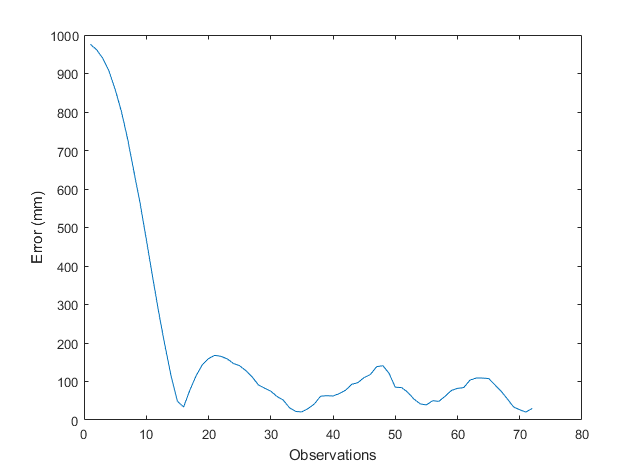
\includegraphics[width=60mm,height=60mm]{Images/kalman_plots/first_dyn_error.png}}
     {Kalman Filter error.}
%\hline
\end{tabular}}
\caption{Dynamic - 1: Q = 0.01 and R = 1.}
\label{fig:kf_dyn1}
\end{figure} 

\begin{figure}[ht!]
\centering
\captionsetup{justification=centering,margin=1cm}
\resizebox{\textwidth}{!}{\begin{tabular}{cc}
%\hline
\subf{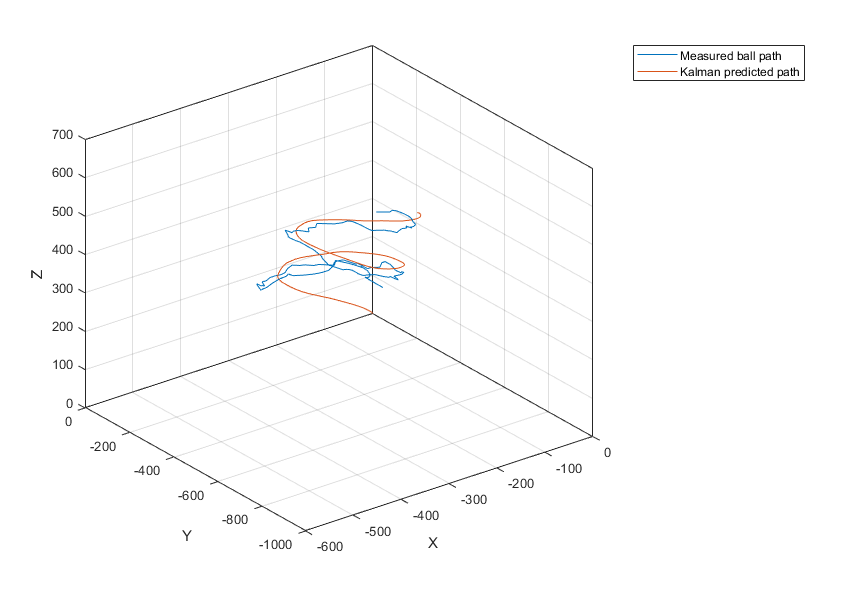
\includegraphics[width=60mm,height=60mm]{Images/kalman_plots/second_dyn_1.png}}
     {KF and Measurements in space.}
&
\subf{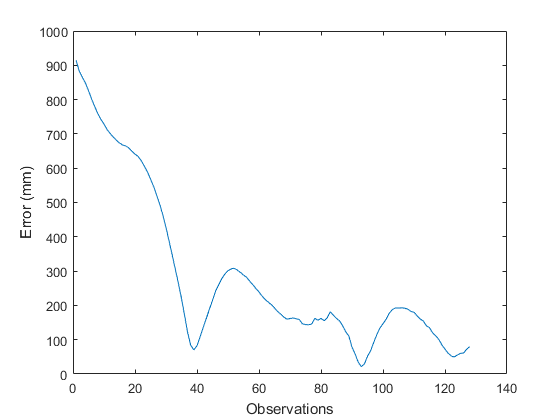
\includegraphics[width=60mm,height=60mm]{Images/kalman_plots/second_dyn_error.png}}
     {Kalman Filter error.}
%\hline
\end{tabular}}
\caption{Dynamic - 2: Q = 0.01 and R = 100}
\label{fig:kf_dyn2}
\end{figure} 

\begin{figure}[ht!]
\centering
\captionsetup{justification=centering,margin=1cm}
\resizebox{\textwidth}{!}{\begin{tabular}{cc}
%\hline
\subf{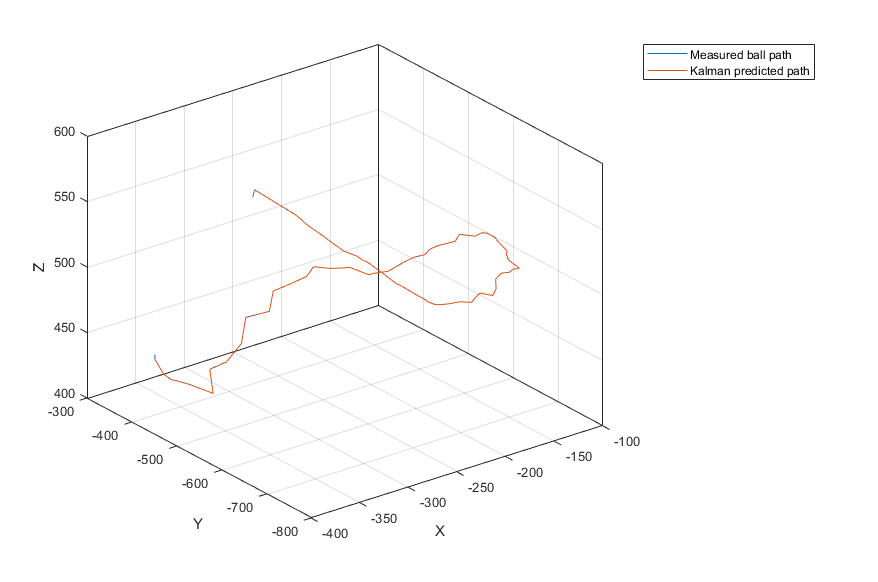
\includegraphics[width=60mm,height=60mm]{Images/kalman_plots/third_dyn_1.png}}
     {KF and Measurements in space.}
&
\subf{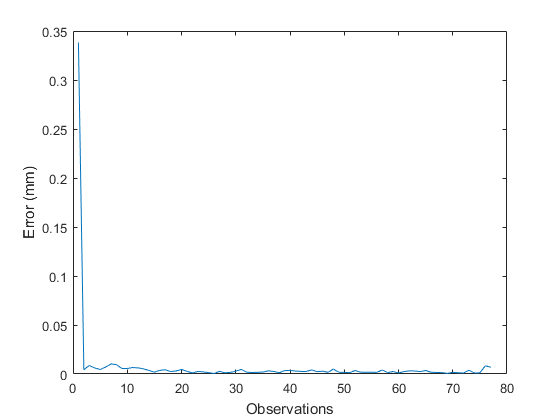
\includegraphics[width=60mm,height=60mm]{Images/kalman_plots/third_dyn_error.png}}
     {Kalman Filter error.}
%\hline
\end{tabular}}
\caption{Dynamic - 3: Q = 200 and R = 0.1}
\label{fig:kf_dyn3}
\end{figure} 

\begin{figure}[ht!]
\centering
\captionsetup{justification=centering,margin=1cm}
\resizebox{\textwidth}{!}{\begin{tabular}{cc}
%\hline
\subf{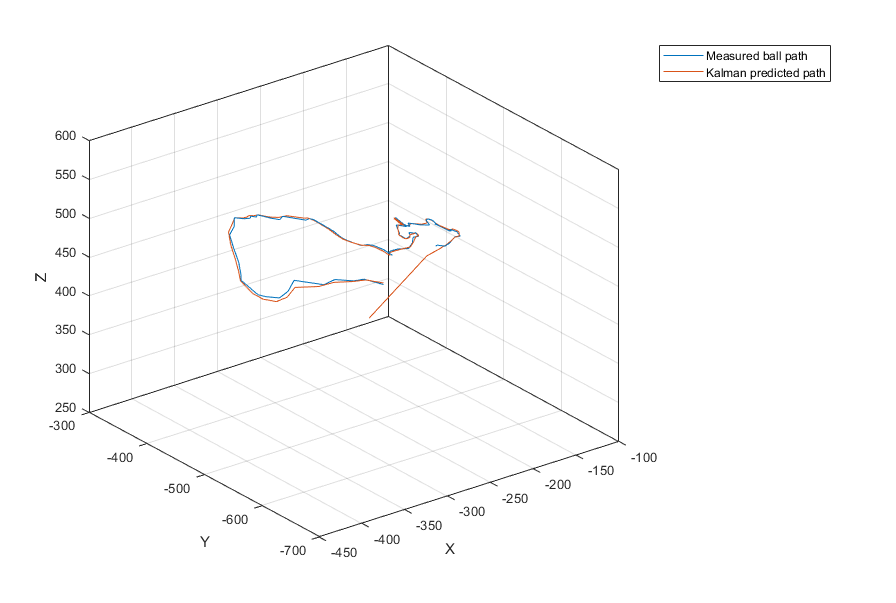
\includegraphics[width=60mm,height=60mm]{Images/kalman_plots/fourth_dyn_1.png}}
     {KF and Measurements in space.}
&
\subf{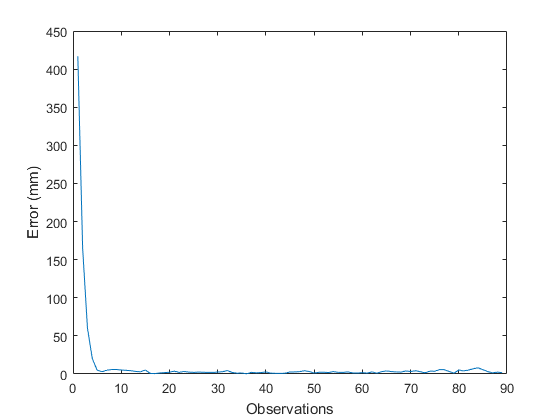
\includegraphics[width=60mm,height=60mm]{Images/kalman_plots/fourth_dyn_error.png}}
     {Kalman Filter error.}
%\hline
\end{tabular}}
\caption{Dynamic - 4: Q = 300 and R = 300.}
\label{fig:kf_dyn4}
\end{figure} 